\subsection{Step 3: Computing the Optimal Cost.}

At this point, we could easily write a recursive algorithm based on recurrence (3) to compute the minimum cost m [ 1, n ] for multiplying $A_{1} A{2} ... A_{n}$. Observe that we have relatively few distinct sub-problems: one sub-problem for each choice of {\itshape i} and {\itshape j} satisfying 1 $\leq$ i $\leq$ j $\leq$ n or ${n \choose k}$ + n = $\theta( n^{2} )$ in all. A recursive algorithm may encounter each sub-problem 2 many times in different branches of its recursion tree. This property of overlapping sub-problems is the second hallmark of when dynamic programming applies (the first hallmark being optimal substructure). Instead of computing the solution to recurrence (3) recursively, we compute the optimal cost by using a tabular, bottom-up approach. \hfill \break

We shall implement the tabular, bottom-up method in the procedure {\bfseries matrix$\_$chain$\_$order}, which appears below. This procedure assumes that matrix $A_{i}$ has dimensions $p_{i-1} x p_{i}$ for {\itshape i = 1, 2, ..., n} . Its input is a sequence $p\ =\ \langle\ p_{0},\ p_{1},\ ...,\ p_{n}\ \rangle$ where {\itshape p.length = n + 1}. The procedure uses an auxiliary table m [ 1 ... n, 1 ... n ] for storing the m [ i, j ] costs and another auxiliary table s [ 1 ... n - 1, 2 ... n ] that records which index of {\itshape k} achieved the optimal cost in computing m [ i, j ]. We shall use the table {\itshape s} to construct an optimal solution. In order to implement the bottom-up approach, we must determine which entries of the table we refer to when computing m [ i, j ]. Equation (3) show that the cost of m [ i, j ] of computing a matrix-chain product of {\itshape j - i + 1} matrices depends only on the costs of computing matrix-chain products of fewer than {\itshape j - i + 1} matrices. This is, for {\itshape k = i, i + 1, ..., j - 1}, the matrix $A_{i ... k}$ is a product of {\itshape k - i + 1 $<$ j - i + 1} matrices and the matrix $A_{k + 1 ... j}$ is a product of {\itshape j - k $<$ j - i + 1} matrices. Thus, the algorithm should fill in the table m in a manner that corresponds to solving the parenthesization problem on matrix chains of increasing length. For the subproblem of optimally parenthesizing the chain $A_{i} A_{i+1} ... A_{j}$, we consider the sub-problem size to be the length {\itshape j - i + 1} of the chain. \hfill \break

\begin{lstlisting}
def matrix_chain_order ( p ):
    n = len ( p )
    # Initialize the matrices of size n x n.
    m = [ [ "x" for i in range ( 1, n + 1 ) ] for j in range ( 1, n + 1 ) ]
    s = [ [ "x" for i in range ( 1, n + 1 ) ] for j in range ( 1, n + 1 ) ]
    # m [ i, i ] = 0 for i = 1, ..., n (minimum costs for chains of length 1).
    for i in range ( n ):
        m [ i ] [ i ] = 0
    # Finds the optimal matrix-chain product.
    for l in range ( 2, n ):
          for i in range ( 1, n - l + 1 ):
              j = i + l - 1
              m [ i ] [ j ] = int ( 1e100 )
              for k in range ( i, j ):
                  q = m [ i ] [ k ] + m [ k + 1 ] [ j ] + (p[ i - 1 ]*p[k]*p [j])
                  if ( q < m [ i ] [ j ] ):
                      m [ i ] [ j ] = q
                      s [ i ] [ j ] = k
                      
	return m, s
\end{lstlisting} \hfill

\begin{figure}[H]
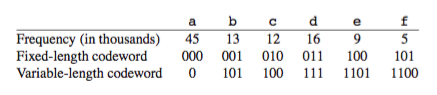
\includegraphics[height = 5cm, width = 16.5cm]{1.png}
\centering \linebreak \linebreak {\itshape\small Figure 3.3.0: The {\itshape m} and {\itshape s} tables computed by {\bfseries matrix$\_$chain$\_$order} for n = 6 and the matrix dimensions in table 1. The tables are rotated so that the main diagonal runs horizontally. The m table uses only the main diagonal and upper triangle, and the s table uses only the upper triangle. The minimum number of scalar multiplications to multiply the 6 matrices is m [ 1, 6 ] = 15, 125.}
\end{figure}

\begin{center}
\begin{tabular}{c c c c c c c}
\toprule
\toprule
\hspace{5px} Matrix \hspace{5px} & \hspace{20px} $A_{1}$ \hspace{20px} & \hspace{20px} $A_{2}$ \hspace{20px} & \hspace{20px} $A_{3}$ \hspace{20px} & \hspace{20px} $A_{4}$ \hspace{20px} & \hspace{20px} $A_{5}$ \hspace{20px} & \hspace{20px} $A_{6}$ \hspace{20px} \\
\toprule
\toprule
Dimensions & 30 x 35 & 35 x 15 & 15 x 5 & 5 x 10 & 10 x 20 & 20 x 25 \\
\bottomrule
\end{tabular}
\linebreak \linebreak Table 1: Matrices dimensions for Figure 3.3.0.
\end{center} \hfill \break

The algorithm first computes m [ i, i ] = 0 for {\itshape i = 1, 2, ..., n}  (the minimum costs for chains of length 1) in lines 7 - 8. It then uses recurrence (3) to compute m [ i, i + 1 ] for {\itshape i = 1, 2, ..., n - 1} (the minimum costs for chains of length l = 2) during the first execution of the {\bfseries for} loop in lines 10 - 18. The second time through the loop, it computes m [ i, i + 2 ] for {\itshape i = 1, 2, ..., n - 2} (the minimum costs for chains of length l = 3), and so forth. At each step, the m [ i, j ] cost computed in lines 15 - 18. Depends only on entries m [ i, k ] and m [ k + 1, j ] already computed. \hfill \break

Figure 3.3.0 illustrates this procedure on a chain of n = 6 matrices. Since we have defined m [ i, j ] only for i $\leq$ j, only the portion of the table m strictly above the main diagonal is used. The figure shows the table rotated to make the main diagonal run horizontally. The matrix chain is listed along the bottom. Using this layout, we can find the minimum cost m [ i, j ] for multiplying a sub-chain $A_{i} A_{i+1} ... A_{j}$ of matrices at the intersection of lines running northeast from $A_{i}$ and northwest from $A_{j}$. Each horizontal row in the table contains the entries for matrix chains of the same length. {\bfseries matrix$\_$chain$\_$order} computes the rows from bot- tom to top and from left to right within each row. It computes each entry m [  i, j ] using the products $p_{i-1} x p_{k} x p_{j}$ for {\itshape k = i, i + 1, ..., j - 1} and all entries southwest and southeast from m [ i, j ].

\pagebreak